\documentclass[a4paper,12pt]{report}
\usepackage[utf8]{inputenc}

\usepackage[unicode,colorlinks,linkcolor=blue,urlcolor=blue]{hyperref}

\PassOptionsToPackage{defaults=hu-min}{magyar.ldf}
\usepackage[magyar]{babel}
\usepackage{graphicx}
\usepackage{textgreek}
\usepackage[delims]{lgreek}
\usepackage{couriers}
\usepackage{amssymb}

\usepackage[top=25mm, bottom=25mm, left=35mm, right=25mm]{geometry}
\usepackage{setspace}

\sloppy
\linespread{1.5}

\begin{document}

% Title Page
%\title{Diplomacím}
%\author{Hack János}
%\date{2015. május}
%\maketitle

\begin{titlepage}

\begin{center}

{\sc \LARGE Eötvös Loránd Tudományegyetem}\\[0.7cm]
{\sc \Large Informatikai Kar}\\[0.7cm]
{\sc \large Programozási Nyelvek és Fordítóprogramok Tanszék}\\[1cm]

\includegraphics[width=0.3\textwidth]{elte_cimer_szines}\\[1.0cm]


{\bf \huge C++ kódgenerálás futtatható UML modellekből}\\[0.5cm]
%{\bf \huge struktúrált megjelenítése}\\[1.5cm]

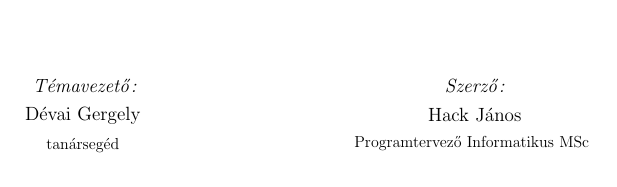
\includegraphics[width=1.1\textwidth]{cimlap.png}\\[1.0cm]

Budapest, 2015

\end{center}

\end{titlepage}

\tableofcontents

\chapter{Bevezetés}

Napjaink szoftverfejlesztésében, az objektum orientált alkalmazások tervezésénél legelterjedtebb módszer az UML\cite{omg2008unified}.
A rendszerek UML-el történő modellezése a programozási nyelvektől független módon képes leírni az elemek kapcsolatát és
viselkedését különböző diagramokon keresztül, amik jól értelmezhető vizuális, formában ábrázolhatóak. Az UML szabvány igyekszik egy rendszer minden aspektusára
valamilyen tervezési eszközt nyújtani, különböző diagramok formájában. Ezek közül a diagramok közül a legelterjedtebbek az osztály és állapotgép diagramok,
valamint a rendszer időbeni viselkedésének leírására szolgáló szekvencia diagramok. A tervezés szakaszának lezárultával a diagramok már csak a rendszer szerkezetét
őrzik. Az elkészítendő szoftver további részei, a függvények, eljárások törzse az objektum példányosítások és a működés implementálása a cél programozási nyelven történik.

Az UML szabvány fejlődésével lehetőség nyílik végrehajtható UML modellek létrehozására is. Egy ilyen új szabvány az fUML \cite{fum}, ami az aktivitásokhoz formálisan definiál végrehajtási szemantikát.
A működési szemantikával lehetővé válik a rendszer működésének szimulálása, aminek segítségével a fejlesztés korai szakaszában felfedezhetővé válnak a specifikáció vagy annak téves értelmezéséből származó hibák. A modellek futtatása történhet automatikusan, ezzel lehetővé téve a hatékony tesztelést, illetve manuálisan, lépésenként, a hibák hatékonyabb megtalálása, vagy a rendszer működésének könnyebben megérthetősége érdekében. Ehhez azonban szükség van valamilyen akció leíró módszerre, egy akció nyelvre, vagy az UML-ben megtalálható aktivitás diagramra.

A modell megalkotásával és a működésének tesztelésével még nem készül el a szoftverünk, mivel azt valamilyen platformra kell majd telepítenünk és futtatnunk. Erre két megoldás létezik, vagy írunk egy virtuális gépet a platformokra, ami képes az UML modell-t futtatni és így működik a szoftver, vagy futtatható kódot generálunk belőle, egy már használt programozási nyelven. Az UML osztály és állapotgép diagramjából történő kódgenerálást számos szoftver támogatja, azonban az aktivitásokból történő generálás és utána a rendszer megfelelő szemantikával történő futtatása csak kevés esetben, vagy egyáltalán nem támogatott.

A dolgozatban a modellből történő teljes kódgenerálással foglalkozunk, különös tekintettel a dinamikus viselkedést leíró állapotgép és aktivitás diagramokkal, valamint a generált kód megfelelő szemantikával történő futtatásával.
A generálás célnyelve a C++. A dolgozatban használt módszer az állapotgépek esetén nem alkalmazható más nyelvekre, azonban az aktivitás diagramok feldolgozására leírt algoritmusok nyelvfüggetlenek.
Az így generált kód megfelelő szemantikával történő futtatására adunk egy futtató környezetet, ami általánosan alkalmazható más állapotgép modellekel is, a megfelelő leszármaztatások implementálása után. 
Az elméleti eredményeink alkalmazásra kerülnek a mellékelt programban, ami a megfelelő UML modellekből C++ kódot készít. A dolgozat további részében bemutatjuk a már létező generálási módszereket, szoftvereket. 
Megvizsgálunk a C++ nyelvhez már létező állapotgép leírást lehetővé tevő könyvtárakat, majd leírjuk a saját munkánkat.
A legvégén pedig a futtató környezet segítségével végzett méréseinkről számolunk be és értékeljük az általunk leírt módszereket.

\chapter{Irodalmi áttekintés}

A kódgenerálás UML osztály diagramokból minden tervező eszköz által támogatott, ami tartalmaz kódgenerálási funkciót. Az így generált kód tartalmazza az osztályok vázát, a metódusokat, adattagokat. Az ehhez szükséges információk kinyerése és helyes összeillesztése egy
osztály vázává nem jelent kihívást a mai eszközökkel, egyszerűen csak be kell járni a modellt és sorban beilleszteni a kódrészleteket. Az adattagok sorrendje ugyan megváltozhat a generáláshoz felhasznált metamodell függvényében, de ez nem befolyásolja a kód funkcionalitását,
csak a felhasználónak okozhat kényelmetlenséget, hogy megtaláljon egy keresett adattagot, vagy függvényt az osztályban. A sorrend változásától és egyéb olvashatósági szempontoktól, sorok tördelése, a behúzások mértéke, eltekintve az elkészült kód nagy része megegyezik a különböző eszközökkel történő generálás esetén. A piac egyik legelterjedtebb eszköze az {\bf EnterpriseArchitect}\cite{ea}, ami több nyelvre is nyújt kódgenerálási lehetőséget, jó kiindulási alapként szolgál, ha ilyen eszközöket keresünk.

\section{Állapotgépekből történő kódgenerálás}

A modellben szereplő állapotgépekből történő kódgenerálása azonban már nem triviális feladat. Különböző módszerek léteznek az egyes elemek (állapotok, átmenetek, átmeneti feltételek, összetett állapotok) feldolgozására \cite{AMT} 
a cél függvényében. A három gyakorlatban is alkalmazott eljárás a következő:
\begin{enumerate}
\item Állapot tervminta\cite{ERRJ:Design} alkalmazása.
\item Logikaként történő elkódolás.
\item Adatként történő elkódolás.
\end{enumerate}
Mielőtt kiválasztanánk az általunk felhasznált ábrázolást, vizsgáljuk meg, milyen tulajdonságokkal rendelkeznek a felsorolt módszerek!


\subsection{Állapot tervminta alkalmazása}

A legelterjedtebb módszer, egy objektum orientált nyelvre történő fordítás esetén az állapot tervmintát
használja fel. Az állapot minta alkalmazása esetén a gép minden állapota egy objektumként van ábrázolva és amikor állapotot váltunk, akkor kicseréljük az aktuális állapotra történő hivatkozást. A belépési és kilépési akciók kezelése a váltásnál történik. A csere kétféleképpen történhet. Az egyik esetben minden alkalommal,
amikor állapotot váltunk, újra létrehozzuk az új állapot objektumát és törüljük a régit. A másik esetben eltároljuk az állapotokat és egy tábla segítségével választjuk ki a megfelelő új állapot objektumot. Egy lehetséges harmadik megoldás a két módszer ötvözése. Amikor egy új, még
nem elért állapotba lépünk létrehozzuk a szükséges objektumot. Ezek után, ha állapot váltásra kerül sor, nem töröljük az állapot objektumunkat, hanem eltároljuk egy táblában és ha újra bele lépnénk, akkor nem hozzuk újra létre, csak kikeressük a már létező állapot objektumot. Az első megoldás a memóriahasználatot a második a futási sebességet részesíti előnyben, míg a harmadik megoldás a kettőt kombinálva próbál egy köztes megoldást nyújtani. A harmadik módszer ugyan átmegy a másodikba, miután minden állapot szerepelt legalább egyszer, de ha van néhány nagyon gyakori állapotunk és a többi csak elenyésző esetben válik aktívvá, akkor ez a módszer összességében hatékonyabb futást eredményez. Az állapot minta alkalmazása esetén az állapot általánosítás és a régiók kezelésére is több megoldás létezik. A régiókkal mi nem foglalkozunk a dolgozatban az állapot általánosítást viszont lehetővé tesszük.

Az összetett állapot egy olyan állapot, ami tartalmazhat további állapotokat vagy maga is állapotgép. Ebben az esetben vagy az állapot objektumai egyben állapotgép objektumok is, és képesek események kezelésére, vagy kiemeljük a belső állapotokat és behúzzuk a szükséges átmeneteket. A kiemelés használata hamar kombinatorikus robbanáshoz vezet és kezelhetetlen méretű állapotgépeket kapunk az átmenetek száma miatt, ezért ez a megoldás csak korlátozott körülmények között alkalmazható.(lásd 2.1 ábra)

\begin{figure}[hbtp]
\centering
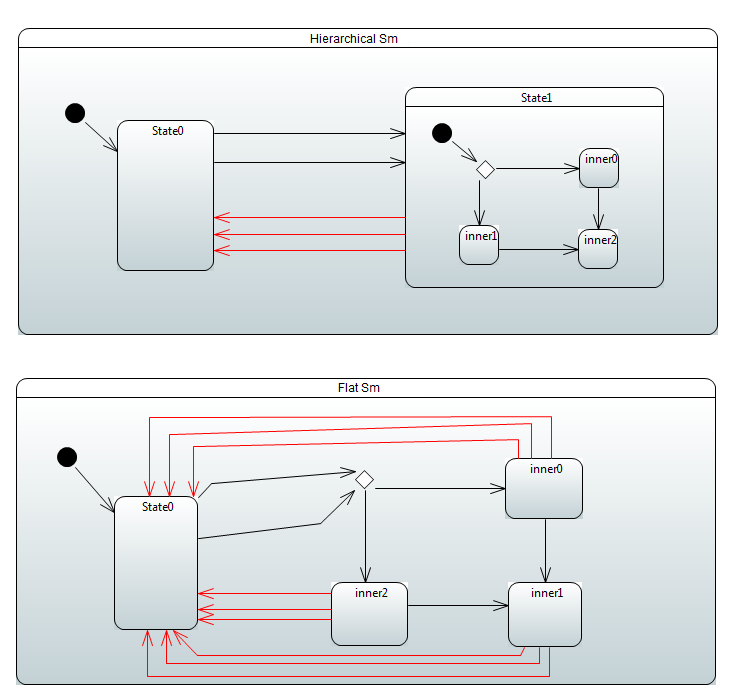
\includegraphics[width=0.76\textwidth]{hierflatcol.png}
\caption{Öszettet állapotot tartalmazó vs Egyszerű állapotgép}
\label{fig:he}
\end{figure}

\subsection{Logikaként történő elkódolás}

A logikaként történő elkódolás a memória használatot igyekszik minimalizálni a program által tárolt adatok csökkentésével, a futási idő és a programkód hosszának rovására.
Ebben az esetben az állapotgép elágazások segítségével kerül elkódolásra, ami jelentős mértékben megnöveli a generált kód hosszát és rontja az átláthatóságot, ezzel megnehezítve a hibakeresést. Továbbá nagyméretű állapotgépek esetén a módszer már kódhosszra vonatkozó korlátokba is ütközhet. A futási időt befolyásolja az állapotgép elkódolása, hogy milyen sorrendben írjuk a elágazás ágait. A gyakori események és állapotok előre vételével, gyorsítható az elérésük. Bizonyos programozási nyelvek tartalmaznak {\it switch} utasítást, amelyet az okos fordító programok ugró táblára\cite{jt} fordítanak le, amiben indexeléssel választható ki a helyes ág. Ebben az esetben a sebesség csökkenés mértéke mérséklődik, de nem minden eseteben generálódik ilyen tábla és függ a fordító program belső határ értékeitől is, hogy hány ágtól alkalmazza ezt a módszert. % példa C++-ból meg hivatkozás erre az ugró táblára valahonnan

\subsection{Adatként történő elkódolás}

Az állapotgépekből történő kódgenerálásnak egy másik alternatív módszere az állapotgép táblaként történő elkódolása\cite{pilitowski2007code}.
Az adatként történő ábrázolás a futási időt tekinti elsődleges szempontnak, ezzel több, az adatok tárolásához szükséges memóriát igényelve a rendszertől. A programkód hossza ebben az esetben jelentősen rövidebb, mint a logikaként történő elkódolás esetén, így ebben az ábrázolásban könnyebb megtalálni a hibákat. A programkód hosszának jelentős csökkenésével azonban nem nyerünk annyi memóriát, hogy a megnövekedett adatmemóriát kompenzálni tudjuk. A táblát valamilyen gyorsan indexelhető adatszerkezetként szokás ábrázolni. A gyors programfutást, az adatszerkezet elemeinek gyors elérése biztosítja.

Az egyik lehetséges megoldás az állapotgép átmenet táblájának az elkódolása, ahol az események és az állapotok egy mátrix sorainak és oszlopainak a címkéi a táblázat mezőiben pedig a célállapot található. A mezőkben továbbá szerepelhet az átmenethez tartozó feltétel és akció is, ha van.

\begin{figure}[hbtp]
\centering
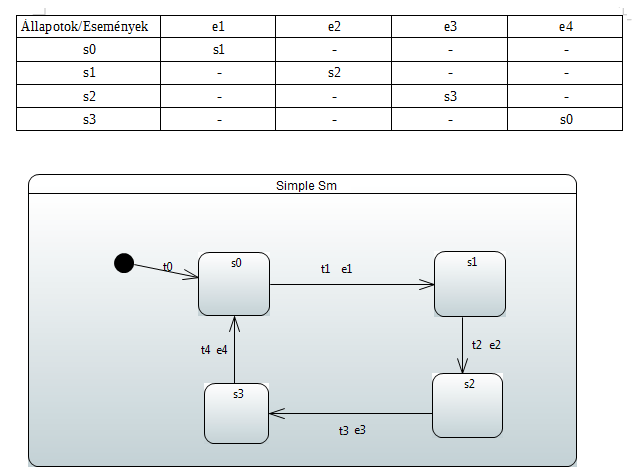
\includegraphics[width=0.75\textwidth]{smtable.png}
\caption{Átmeneti tábla}
\label{fig:at}
\end{figure}

Az események feldolgozása indexelés segítségével történik az aktuális állapot és a kapott esemény alapján. A kapcsoló tábla használata esetén további számításokat jelent, ha egy állapotból ugyanarra az eseményre több másik állapotba is átléphetnénk, ahol az átmenetek csak a feltételben különböznek. Az állapotgépek elkódolása azonban többféleképpen is történhet és a fentebb említett számításokra is megoldás kínálkozik, vagy leszűkíthető a kezelt állapotgépek halmaza.

Összességében az állapotgépek elkódolására több eljárás is alkalmazható, a választott módszer a célkörnyezet és a programtól elvárt tulajdonságoktól függ.

\section{Aktivitások és generálásuk}

Az aktivitások generálása már kevésbé elterjedt a modellező eszközök terén. Azok a programok, amik támogatják már túllépnek a puszta váz modellezésen, és valamilyen végrehajtható UML modellt használnak. További problémát jelent, hogy az aktivitás diagramok szabványa nagyon megengedő és kevés szemantikai/szintaktikai megkötést tesz, ezért az olyan eszközök, amik teljes kódgenerálást támogatnak,
nem minden esetben használják az aktivitás diagramokat, mint akció leíró eszközt. Az {\bf EnterpriseArchitect} támogatja az aktivitás diagramok, sőt a szekvencia diagramokkal történő akció leírást is, de más eszközök mint a {\bf BridgePoint}\cite{bp}
is egy akció leíró nyelvet definiál, aminek segítségével program utasításokhoz hasonló módon tudjuk leírni a funkcionalitást. Az ilyen akció nyelvek az ismert programozási nyelvekhez hasonló utasításokkal és szintaktikával rendelkeznek, így
gyorsan tanulhatóak és hatékonyan használhatóak. A kódgenerálás az ilyen akció leírásból nyelvek közti átalakítással megoldható, valamint az ilyen módon történő akció leírás gyorsan megérthető más fejlesztők által. Az előnyei mellett azonban
számos hátrányos tulajdonsága is van az ilyen megoldásoknak. Az egyik legjelentősebb, hogy nem szabványos. Ugyan vannak törekvések egy szabványos leíró nyelv generálására (fUML), de jelenleg minden eszköz a saját leíró nyelvét használja, ami sérti %más szó
a modell hordozhatóságát és eszköz függetlenségét. Az aktivitás diagramok a fentebb említett leíró nyelvekhez képest kevés előnyös tulajdonságot tudnak felmutatni a megértésük és átlátásuk merőben függ az ember vizuális beállítottságától. Azonban vizuális jellege miatt, akár programozásban nem jártas személyekkel is megértethető a tartalma. A diagram előállításának sebessége is változó és nagyban befolyásolja a használt eszköz minősége. Az előállítás sebessége minden esetben lassabb, mint egy akció nyelvvel történő azonos kód előállítása. A megírt kód hibajavítása az aktivitás diagramok esetén azonban könnyebb lehet mint az akciónyelv hibajavítása.
A fentebb leírtak alapján, az akció nyelv gyorsabb és hatékonyabb fejlesztést nyújt feltéve, hogy ragaszkodunk egy választott eszközhöz és annak minden előnyéhez és hátrányához, míg az aktivitás diagramok esetén tetszőleges végrehajtható UML-t támogató eszközt használhatunk a fejlesztésére.
Az aktivitás diagramokból történő kódgenerálásról publikált munkák\cite{bjorklund2004unified,eshuis2001execution}
nem nyújtanak jól alkalmazható módszert. Az eszközök, amik pedig támogatják, mint például az { \bf Enterprise Architect} üzleti alkalmazások, amiknek a kódja zárt és az alkalmazott módszerek céges titkok.

\section{Generált kód futtatása}

Miután a kész szimulációban jól működő modellünkből legeneráltuk a forráskódot, szeretnénk azt, az UML modellünk szimulációjának megfelelő módon futtatni. Ehhez azonban szükségünk van egy futtatási környezetre, ami biztosítja az események kezelését és az állapotgépek működését a valamilyen végrehajtható UML szimulációval azonos módon \cite{EPC}.
A piacon lévő kódgenerálásra képes eszközöknek csak egy nagyon kis százaléka ad a generált kódhoz futtatási környezetet. Legtöbb esetben csak legenerálják a dinamikus működéshez tartozó elemeket és a felhasználóra bízzák a további lépéseket, hogy hogy használja fel a generált állományokat. A dolgozatban fontosnak tartjuk a cél nyelven történő szimuláció problémájának a lefedését, mivel a kódgenerálás végső célja az elkészült kód felhasználása és futtatása.
Ahhoz hogy ezt megtegyük szükségünk van a szimulációs szemantikára, amivel a modellt a generálás előtt teszteltük és készítenünk kell egy futtatási környezetet, ami képes azonos viselkedést nyújtani a generálás célnyelvén. A továbbiakban a modellek által használt futtatási szemantikával foglalkozunk.

\subsection{Futtatási szemantika és felhasználható elemek}%átfogalmazni

%berakni azt hogy milyen nevei lehetnek az elemeknek, hogy a c++ kód fordítás ne akadjon fenn rajtuk
Az UML szabvány nem foglalkozik a modellek futtatásával, így nem ad futtatási szemantikát a szimulálásukhoz. A végrehajtható UML fejlődésével azonban több munka is született a lehetséges futtatási szemantikákról\cite{storrle2004semantics,mellor2002executable,harel2004rhapsody,von2002structured}.
Az általunk használt szemantika és a kódgenerálás dolgozatban leírt elméletét felhasználó program egy fejlesztés alatt álló eszközben kerül alkalmazásra a {\bf txtUML}\cite{txtuml}-ben, ezért bizonyos megkötéseket teszünk az állapotgépekben és aktivitásokban alkalmazható elemekre az eszköz a dolgozat elkészülésének idejében lévő állapota alapján. Az állapotgépekben jelenleg nem kapnak helyet az alábbi elemek:
\begin{itemize}
\item {\it history}.
\item {\it regions}.
\item {\it junction}.
\end{itemize} 
Az átmeneteken nem használhatunk {\it Time}, {\it Call} valamint {\it ChangeEventet}.
Az állapotgépekben megengedett elemek:
\begin{itemize}
\item egyszerű állapotok.
\item összetett állapotok.
\item belépési és kilépési akciók.
\item egyszerű átmentek valamilyen szignál esemény hatására.
\item elágazások.
\item átmenti feltételek.
\item átmeneti akciók.
\end{itemize}
Az akciókban az elemek száma miatt a megengedett elemek felsorolása az eszköz dokumentációjában található, az állapotgépekben megengedett elemek pontos listájával.
Az állapotgépekben az események kezelése a következőképpen történik:
\begin{enumerate}
\item Megvizsgáljuk, hogy van-e az adott állapotban olyan átmenet aminek az esemény hatására tüzel. Az átmeneteket, ha összetett állapotban vagyunk a legbelső állapottól kifelé kezdjük el vizsgálni.
\item Ha találunk olyan átmentet aminek az esemény hatására kell tüzelnie és az átmeneten szereplő feltétel is teljesül akkor végrehajtjuk az aktuális állapot kilépési akcióját. Ezután az átmenetei akció majd a cél állapot belépési akciói, összetett állapot esetén kívülről befelé haladó sorrendben hajtódnak végre.
\item Ha nem találunk az esemény hatására tüzelő átmentet, vagy egyik átmeneti feltétel sem teljesül, akkor eldobjuk az eseményt.
\end{enumerate}
Az események feldolgozása sorban történik. Egy esemény feldolgozása közben az érkező új események bekerülnek az állapotgép esemény sorába. Az elküldött események sorba kerülésének sorrendje nem meghatározott, a futtatási környezettől függ, de a dolgozatban leírt környezetben lehetőség lesz determinisztikus futtatásra is.
A késleltetett vagy {\it deferred}, események nem támogatottak. Az akciókban és a feltételekben alkalmazhatunk OCL\cite{omg20052}
leírásokat is korlátozott körülmények között. A teljes OCL nyelv támogatása kívül esik a dolgozat keretein.
Az állapotgépek állapota kizárólag események hatására változhat meg. Az állapotgép önmagának küldött eseménye nem élvez prioritást, minden esemény a sorba kerülésének rendjében kerül feldolgozásra. Az állapotgépek párhuzamosan futnak, minden állapotgép saját eseménysorral rendelkezik. Az aktivitások végrehajtása megszakíthatatlan. Minden aktivitásnak rendelkeznie kell egy kezdeti és vég ponttal és csak eggyel. Az aktivitások felhasználhatják a kiváltó esemény paramétereit, de nem változtathatják meg azokat. Az aktivitások kizárólag az állapotgép és annak adattagjait módosíthatják. Az akciók tartalmazhatnak ciklusokat és elágazásokat az alábbi szintaktikai szabály betartása mellett: Az elágazás, vagy ciklus kezdetét egy elágazás pszeudo csúcs jelzi. Az elágazás esetén minden ágnak egy elágazás záró pszeudo csúcsban kell találkozni és léteznie kell egy különben ágnak, ami biztosítja a tovább haladást a feltételek nem teljesülése esetén is.
A ciklusból pontosan egy ágnak kell kivezetnie. A többi ág mind a ciklus kezdeti csúcsában kell hogy végződjön.

A fentebb leírt szabályok betartásának eleget tévő modellekre biztosítjuk a dolgozatban később leírt módszerek működését és a fejezetben leírt szemantikai szabályok betartását a futtatási környezet használata esetén.

\section{Létező könyvtárak}

Mielőtt elkészítenénk a kódgenerálásnál használandó saját állapotgép ábrázolásunkat, vizsgáljuk meg, milyen már létező C++ könyvtárakat tudnánk felhasználni.

\subsection{Boost::Statechart}

A Statechart könyvtár \cite{donni2007boost} egy gyors, közvetlen C++-ra történő átírást tesz lehetővé az UML-ben leírt állapotgépekből. A könyvár template metaprogramozás és az állapot minta alkalmazásával oldja meg a feladatot. Mind az állapotgépeknek, mind az állapotoknak van egy ős osztálya, ami több template paramétert vár. Az első paraméter mind esetben maga a leszármazott osztály típusa a curiously recurring\cite{coplien1995curiously} template minta alapján. %lehet kép erről
A további paraméterek változóak az állapotgép esetén a kezdeti állapot, amibe a gép lép inicializálás után az állapotnál a kontextus amiben használjuk. A kontextus lehet:
\begin{itemize}
\item Az állapotgép, amiben az aktuális állapot szerepel.
\item Egy állapot, aminek egy belső pontja az elem.
\item Egy régió, amibe az elem beletartozik. 
\end{itemize}
A kilépési és belépési akciók az állapot osztály konstruktora és destruktoraként valósíthatóak meg, a könyvtár működési elvének köszönhetően ugyanis egy állapot objektum csak addig él, amíg aktuális állapot. Az állapot váltás törli a régi és létrehozza az új állapotnak megfelelő objektumot. Az állapotgépek létrehozásuk után nem egyből aktívak. El kell őket indítani az {\it initiate} függvény meghívásával. Az átmeneteket az állapotokban kell definiálnunk. Többféle átmenetet definiálhatunk. Az első és legegyszerűbb átment nem tartalmaz semmi mást csak egy eseményt, aminek hatására átlépünk egyik állapotból a másikba. Ennek a leírása legegyszerűbben a következőképpen tehető:

\begin{figure}[hbtp]
\centering
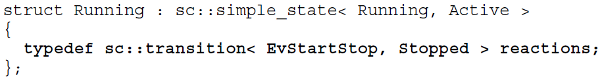
\includegraphics[width=0.8\textwidth]{scst.png}
\caption{Egyszerű átmenet minta}
\label{fig:srtst}
\end{figure}

Az ilyen átmenetek egy valós rendszerben elenyésző mennyiségben vannak jelen. Továbbá, mivel az ilyen definíció tempalte példányosítással jár, nagyobb állapotgépek esetén hamar beleütközünk a fordító példányosítási határába. A definíció sablon mivolta miatt a fordítónak látnia kell minden érintett osztály teljes definícióját a példányosítás érdekében, aminek következtében az egész állapotgép kódja egy fordítási egységbe kell hogy essen, ezzel akadályozva a csapatmunkát is.
Az átmenetek definiálásának másik módja mind a két imént említett problémára megoldást nyújt és lehetővé teszik az összetettebb, valós környezetben is használt gépek implementálását. Ebben az esetben az átmentet csak egy felhasználó által definiált reakció és a kiváltó esemény segítségével definiáljuk a következő módon: 

\begin{figure}[hbtp]
\centering
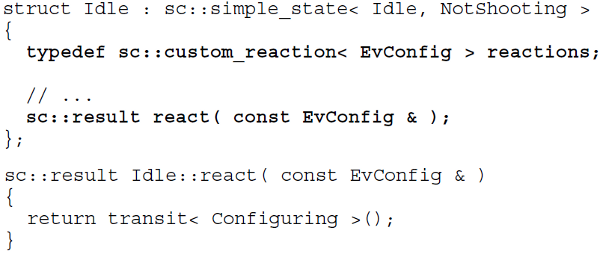
\includegraphics[width=0.8\textwidth]{stcr.png}
\caption{Felhasználó által definiált reakció minta}
\label{fig:stsfl}
\end{figure}

A végrehajtandó akciót a megfelelő paraméterű {\it react} függvény segítségével tudjuk definiálni az osztályban.
Ennek a fajta átment leírásnak a segítségével már szét tudjuk választani az állapotgépünket több fordítási egységre és megadhatunk átmeneti akciókat, feltételeket. Az átmeneti feltételek elágazások formájában adhatóak meg a felhasználó által definiált egyéni reakció törzsében. Az akció visszatérési értéke a {\it result} típus, ami vagy egy átmenet, vagy egy esemény továbbítása magasabb szintre, összetett állapot esetén. Átmenettel történő visszatérési érték esetén ügyelnünk kell arra, hogy azt ezt megvalósító kód után, már semmilyen utasítás ne szerepeljen, amit végre akarnánk hajtani, mivel az átmenet egyenértékű az objektum törlésével. 

A könyvtár továbbá lehetővé teszi több reakció kezelését is, ebben az esetben a {\it reactions} típus egy template meta lista, amiben a különböző átmeneteket tároljuk. Az állapot minta használatának további következményeként az állapotokban tárolt adatok élettartama megegyezik az állapotgépével, így a kinyerésükhöz az állapotgépen szükségünk van különböző függvényekre. A könyvtár erre a {\it state\_cast} függvényt biztosítja a számunkra. Ha meghívjuk a függvényt az aktuális állapottal, mint paraméterrel, akkor visszakapjuk az állapot objektumot, különben {\it bad\_cast} kivétel keletkezik.
A könyvtár továbbá lehetőséget ad arra, hogy rákérdezzünk az aktuális állapotra, azonban ezt egy igen, nem választ adó függvény segítségével teszi. A függvény igen választ ad ha a paraméterben átadott állapotban vagyunk különben nem el tér vissza. A Boost::Statechart az összetett állapotokon túl megengedi a régiók használatát is. Az ilyen állapotgépekben egyszerűen csak több kezdeti állapotot kell megadnunk és a régiók állapotainak a régió számát kell átadnunk, amiben szerepelnek, lásd 2.3 ábra.

\begin{figure}[hbtp]
\centering
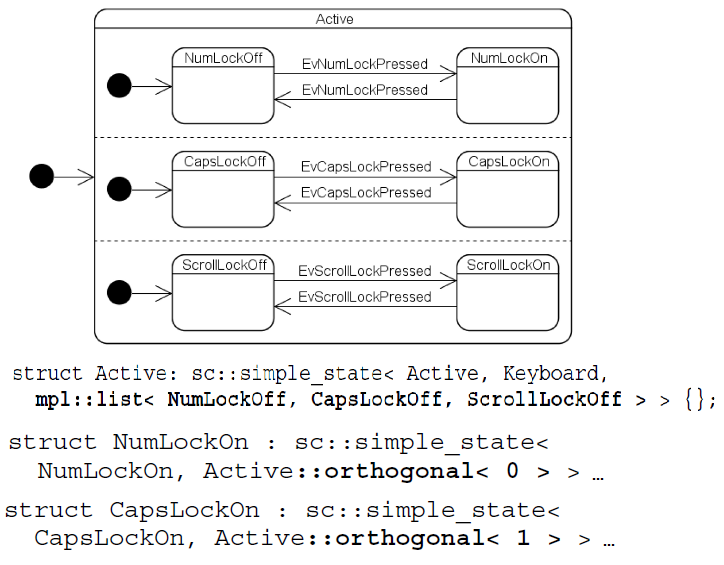
\includegraphics[width=0.9\textwidth]{ortocode.png}
\caption{Ortgonális állapotok leírása}
\label{fig:ort}
\end{figure}

A könyvtár továbbá támogatja a különböző {\it history}-kat is, de ezzel mi nem kívánunk foglalkozni.
A könyvtárral leírható állapotgépek megvizsgálása után vessünk egy pillantást az események kezelésre. Az események kezelése mindig lentől felfelé történik, figyelembe véve az összetett állapotokat és régiókat is. A 2.6-os ábrán látható állapotgép esetén az {\it Ev} esemény feldolgozása a következő függvényhívási sorozattal jár: \begin{math}\thicksim\end{math}D(), \begin{math}\thicksim\end{math}C(), \begin{math}\thicksim\end{math}B(), \begin{math}\thicksim\end{math}A(), t(), X(), Y(), Z().

Az állapotgépek leírásának további megkötése, hogy kívülről befelé kell haladnunk az elemek definiálásával a könyvtár template természetéből kifolyólag a részletes indoklást a fejlesztő által írt tutoriálban olvashatjuk. A könyvtár továbbá támogat kivétel kezelést, amivel szintén nem foglalkozunk.

\begin{figure}[hbtp]
\centering
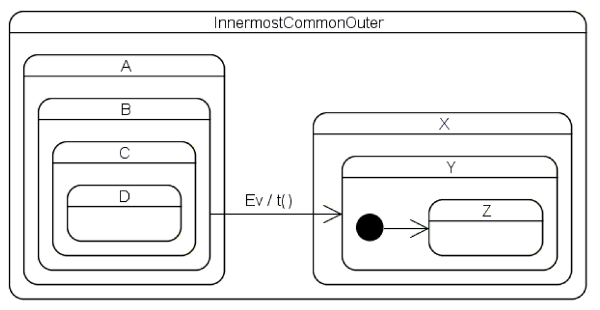
\includegraphics[width=0.75\textwidth]{hier.png}
\caption{Összetett állapotot tartalmazó állapotgép}
\label{fig:hir}
\end{figure}

Összefoglalva a könyvtár tulajdonságait:
\begin{itemize}
\item Előnyők:
\begin{itemize}
\item Könnyű UML-ben leírt állapotgépeket leírni vele
\item Kevés adat memóriát használ
\item Sok UML featuret támogat
\end{itemize}
\item Hátrányok
\begin{itemize}
\item Nem rendelkezik nem template ősosztállyal, az állapotgépek ősosztályon keresztüli polimorfikus tárolása nem biztosított.
\item A használata körülményes mivel template
\item Mivel minden átmenetnél törlés és létrehozás van ezért nem elég gyors
\end{itemize}
\end{itemize}

Összességében a könyvtár gyors, átlátható UML-ből C++-ra történő programozói állapotgép átírásra, de kódgenerálásra nem ajánlott. 

\subsection{Boost::MSM}

A Boost::MSM\cite{henry2008meta} egy másik C++-os állapotgép leíró könyvtár, aminek segítségével gyorsan tudunk állapotgépeket UML-ből átríni. A könyvtár a futási sebességre helyezi a hangsúlyt és ezt template metaprogramozás erőteljes használata segítségével éri el. A könyvtár alap ötlete, hogy az állapotgépet az átmeneti táblájával írja le . 

\begin{figure}[hbtp]
\centering
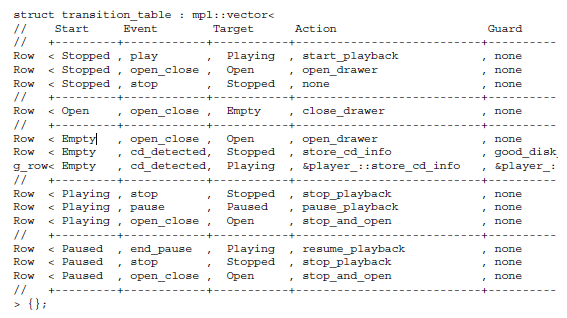
\includegraphics[width=1\textwidth]{msmtable.png}
\caption{MSM állapotgép tábla}
\label{fig:msmat}
\end{figure}

Az MSM ezzel a leírással már közelebb kerül a tényleges kódgeneráláshoz. Annak is az állapotgép adatként történő leíró módszeréhez. A könyvtár két részre bontható. Az egyik a {\it frontend}, ami az állapotgépek leírási módszere. A másik a {\it backend}, ami az állapotgépek működését biztosítja. Jelenleg három {\it frontend} és egy {\it backend} létezik, amiket használhatunk. Vizsgáljuk meg először a különböző állapotgép leírási lehetőségeinket.

Az állapotgép minden esetben egy {\it template meta vektor}-ként van ábrázolva, aminek a sorainak a feltöltésében térnek el a {\it frontendek}. A táblázat soraiban az információkat a következő sorrendben adhatjuk meg:
\begin{enumerate}
\item {\bf Kiinduló állapot}, ahol az állapotgépnek állnia kell, hogy az eseményt kezelje.
\item {\bf Esemény}, aminek hatására átmenet történik.
\item {\bf Cél állapot}, ahova átlépünk az esemény hatására.
\item {\bf Állapot átmeneti akció} a végrehajtandó akció az átmenet esetén.
\item {\bf Átmeneti feltétel}, aminek teljesülnie kell hogy az átmenet megtörténjen.
\end{enumerate}
A könyvtár több sortípust biztosít, amiknek a típusparaméterezése az egyes tagok elhagyását teszi lehetővé.

A történetileg első leírási lehetőség az ötlet forrásának a template metaprogramozás könyvbeli állapotgépnek a mintájára függvénymutatókat használ az átmeneti akciók és feltételek megadására.
Az átmenti függvény szignatúrája a következő: 
\linebreak
{\it \bf void method\_name (const event\&)}.%jobb lenne kódként formázni
Vagyis egy eljárás, ami a kiváltó eseményt mint konstanst kapja paraméterül. Az átmeneti feltételek szignatúrája csak a visszatérési értékben tér el, ami egy logikai érték.

Az első és legegyszerűbb {\it fronted} szépség hibáit a függvény hivatkozások használatát igyekszik elkerülni a második leírási módszer, ahol a táblázat soraiba már nem nyers hivatkozások, hanem {\it funktor} osztályok segítségével adhatjuk meg. %lehet hivatkozás a fumnktorra
E megadási módszer alkalmazásához egy külön osztályba helyezhetjük ki az átmeneti akcióinkat és feltételeinket.
Az ilyen {\it funtor}-ok alkalmazására egy másik sor típus áll rendelkezésünkre, ami csak a kezdőbetűk méretében tér el a régi {\it frontend}-beli megfelelőitől. A {\it funktor frontend} továbbá biztosít egy {\it none} előre megírt feltételt, ami a feltétel hiányát jelöli.

A harmadik leírási lehetőség csak kísérleti jellegű, nem kifejlett. Ez a lehetőség egy akció nyelv segítségével írja le a táblázatot, így nem szükséges {\it funktor}-okat vagy külön függvényeket definiálnunk, helyben kifejthetjük a kívánt hatást a táblázat soraiban.
Ennek a {\it frontend}-nek az alkalmazása azonban behoz egy további függőséget a Boost könyvtárnak és jelentősen lassítja a fordítási időt. Az állapotok továbbra is osztályok a belépési és kilépési akciók azonban nem a konstruktor és destruktor segítségével adható meg, hanem a {\bf void on\_entry(Event const\&, Fsm\& )} és {\bf void on\_exit(Event const\&, Fsm\& )} függvényekkel. A könyvtár támogatja a régiókat, az összetett állapotokat és a {\it historyt}-is akár csak a Boost::Statechart. A kezdeti állapotot az {\it initial\_state} típus definíció segítségével tudjuk megadni az állapotgépben. A kívánt {\it frontend} használata teljesen a felhasználóra van bízva, azonban a {\it backend} jelenleg csak egyféle áll rendelkezésre. A logikát az alábbi definíció segítségével tudjuk elérhetővé tenni:

\begin{figure}[hbtp]
\centering
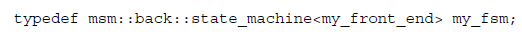
\includegraphics[width=0.8\textwidth]{msmback.png}
\caption{MSM backend típus definició}
\label{fig:msbact}
\end{figure}

Mint a Statechart, esetén ennél a könyvtárnál is kézzel kell az állapotgépeket elindítanunk a {\it start} eljárás hívásával. Az állapotgép futását a {\it stop} hívással tudjuk előidézni, aminek hatására lefut az aktuális állapot kilépési akciója is. A {\it backend} gondoskodik az események kezeléséről. Az események a {\it process\_event} hívásával dolgozhatóak fel. Az eljárás csak konstans eseményeket kezel elkerülve ezzel a mellékhatásokat, az események feldolgozása közben semmilyen más folyamat nem történhet. Az állapotgépek aktuális állapota a {\it current\_state} függvény hívásával eszközölhető, ami az aktuális állapot azonosítóját adja vissza a felhasználónak. A könyvtár továbbá támogatja az állapotgépek szerializációt is. A {\it backend} több lehetőséget is biztosít az állapotgépek működésének változtatására, amiről a dokumentációban a {\it back\_end} szekcióban olvashatunk.
Összefoglalva a könyvtár tulajdonságait:
\begin{itemize}
\item Előnyök:
\begin{itemize}
\item Könnyű UML-ben leírt állapotgépeket leírni vele.
\item Gyorsabb futási idő, mit a konkurens Statechart esetében.
\item Sok UML featuret támogat.
\end{itemize}
\item Hátrányok
\begin{itemize}
\item Mivel sok eleme template a fordítási egységek kialakítása problémát okoz. Nem választható szét a gépek definíciója.
\item A template metaprogramozás használata miatt a fordítási idő kis állapotgépek esetén is nagyon lassú.
\item A táblázat az {\it mpl::vector}-t használja, aminek a mérete limitált, nem alkalmas összetettebb állapotgépek leírására.%lehet kell hivatkozás az mpl::vectorra
\end{itemize}
\end{itemize}

Összességében a könyvtár elég gyors futást eredményez a fordítási időbeni növekedés miatt, azonban csak kis állapotgépek leírása alkalmas mind a metaprogramozásbeli adatszerkezetek mind a fordítási idő növekedés miatt. A kódgenerálásra történő használata nem javasolt a rendkívül hosszú fordítási idő miatt.

\chapter{Modellekből történő kódgenerálás}

\section{válaszotott generálásí módszer}

Az eddig leírt módszerek mindegyike alkalmas UML-ből történő kódgenerálásra. A választást csak az elérendő cél határozza meg. Mivel a dolgozatban a cél nyelv a C++, ezért a futási sebességet részesítjük előnyben a memória használattal szemben, ezért a választott módszer az állapotgép adatként történő elkódolása lesz. 

Az aktivitásokból történő generáláshoz saját algoritmusokat írunk le a terület hiányos irodalma miatt, amik a fentebb leírt szabályokat betartó UML diagramokból helyes kódot generálnak.

\section{Állapotgép generálás}

Az állapotgép elkódolásához négy elem ábrázolására van szükségünk:
\begin{enumerate}
\item {\bf Események}
\item {\bf Állapotok}
\item {\bf Átmeneti akciók}
\item {\bf Átmeneti feltételek}
\end{enumerate}
A továbbiakban sorra vesszük a elemeket és leírjuk, milyen elvárásokat kell teljesíteniük és hogyan oldottük meg ezt C++-ban.

\subsection{Események}

Az állapotgépek generálásánál figyelnünk kell az eseményekre, hogy többalakúak legyenek és egységesen tudjuk őket kezelni. Valamint a gyors valós típus meghatározásra, mivel a gyors futási sebességet tűztük ki célul. Az ős osztálynak tartalmaznia kell valamilyen típus információt, ami alapján azonnal meghatározható a valós esemény. Az események típusa az állapotgép átmenetein is szerepel, ezért ennek a típus információnak az állapotgép számára is felhasználható formában kell szerepelnie a gyors átmenet kiválasztás érdekében. Továbbá a külvilág számara is elérhető kell legyen, hogy biztosítsa az állapotgéppel történő kommunikációt. Minden állapotgép csak egy adott eseménytípus halmazt képes kezelni, ami az átmenetein szerepel és csak azokat. Egy esemény több különböző állapotgép átmenetén is szerepelhet.
A szükséges elvárások teljesítését a C++-ban szereplő felsorolási típus az {\it enum} biztosítja. A felsorolást kétféleképpen tehetjük meg:
\begin{itemize}
\item {\bf Globálisan}: Egy darab felsorolás, ami a modell minden eseményét tartalmazza.
\item {\bf Állapotgéphez kötötten}: Miden állapotgép saját felsorolással rendelkezik az általa elfogadott eseményekről.
\end{itemize}
Mi az állapotgéphez kötött felsorolást választottuk a generálási algoritmus miatt, ami állapotgépenként halad. Valamint a generált kód ellenőrzését is elősegíti ez a megoldás, mivel az állapotgép által elfogadott események és csak azok egy helyen fellelhetőek. Ez a megoldás nem okoz problémát az eseményekben tárolt típus információ megvalósításában, mivel a C++-ban az {\it enum} típus elemei automatikusan konvertálódnak {\it integer} típusú értékekre. Az események típusát egy {\it integer} típusú adattaggal biztosítjuk, aminek a megadása kötelező az esemény létrehozásakor. Az egyetlen hátránya ennek a módszernek, hogy nem típus biztos, két állapotgép különböző eseménye is konvertálódhat azonos számra. Ez a probléma azonban csak hibás modell esetén kerül elő, ahol olyan eseményt akarunk egy állapotgépnek küldeni, amit nem hivatott kezelni. Ennek a hibának a kezelése nem a kódgenerálás feladata, ezért a kód helyes működésének biztosítása ilyen esetben nem elvárható. Az állapotgépek esemény kezelő algoritmusát nem befolyásolja a választott megoldás, így ha szükséges a generáló algoritmus minimális módosításával áttérhetünk a globális, vagy másfajta módszerre. Az egyetlen elvárás, hogy az eseménytípusok számokra konvertálható felsorolási típusként is szerepeljenek. 

Ezek után az eseménykezelés fentebb leírt tulajdonságait a következő ősosztály teljesíti.

\begin{figure}[hbtp]
\centering
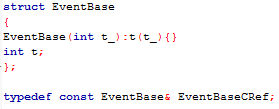
\includegraphics[width=0.5\textwidth]{eventbase.png}
\caption{Esemény Ősosztály}
\label{fig:eb}
\end{figure}

Az események típusonként külön osztállyal rendelkeznek és tetszőleges további adattagokat tartalmazhatnak.

\subsection{Állapotok}

Az állapotok egyszerű esetben semmilyen egyéb információt nem hordoznak mint a gép állását. Egyedül az összetett állapotok azok, amik külön figyelmet igényelnek. A gép aktuális állapotát egy integer típusú változóban fogjuk tárolni az állapotokat pedig felsorolási típusként kódoljuk el az eseményekhez hasonlóan. Az összetett állapotokat úgy kezeljük, mint állapotgépek és külön osztályt hozunk létre nekik. Ahhoz, hogy ezt megtehessük és hogy az állapotgépeinket egységesen tudjuk kezelni bevezetjük a lentebbi ábrán látható ős osztályt.
\begin{figure}[hbtp]
\centering
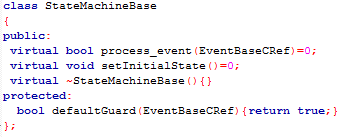
\includegraphics[width=0.6\textwidth]{smbase.png}
\caption{Állapotgép Ősosztály}
\label{fig:smbas}
\end{figure}

Az olyan állapotgépeknél, ahol összetett állapot is szerepel megváltozik az esemény feldolgozó és állapot váltó algoritmus is, amivel az algoritmusok szakaszában foglalkozunk. Az ilyen állapotok tárolásra és jelzésére bevezetünk két további adattagot:
\begin{itemize}
\item {\bf Állapotgép osztály mutató}, ami egyszerű állapotok esetén {\it null} értékű, különben az öszetett állapot objektumra mutat.
\item {\bf Összetett állapotokat tároló adatszerkezet}, aminek segítségével eldöntjük összetett állapotba léptünk-e és tartalmazza az állapot objektumot. Az adatszerkezet egy asszociatív tömb lesz, aminek a kulcsa az állapot felsorolás egy elem, értéke pedig az összetett állapot objektuma.
\end{itemize}
Az összetett állapotok állapotgépként történő kezelése rekurzióval oldja meg a többszöri összetett állapotok problémáját. Az eseménykezelésnél a nehézséget az okozza, hogy a legfelső szinten szereplő állapotgépben kell felsorolnunk az összetett állapotok eseményeit, azonban az összetett állapot osztályokban már nem szerepel további esemény felsorolás. Ezek az osztályok a legkülső tartalmazó gép eseményfelsorolását használják. Probléma az adattagok láthatósága, ugyan is az összetett állapotnak hozzá kell férni a legkülső állapotgép minden adattagjához. A megoldás egy szülő mutató bevezetésével biztosítjuk, amit az állapot létrehozásakor kötelező megadni. A szülő mutató önmagában nem biztosít hozzáférést az adattagokhoz és kényelmi okokból nem {\it set}-erek és {\it get}-erek segítségével szeretnénk ezek elérését biztosítani, így a C++-ban megtalálható {\it friend} mechanizmust használjuk fel megoldásként. A legkülső szülőben minden benne található összetett állapotgépet {\it friend}-nek tüntetünk fel.
Az állapotokkal kapcsolatban nincs további megoldandó problémánk.

\subsection{Átmeneti akciók és feltételek}

Az átmeneti akciók és a feltételek az állapotgép szempontjából csak a futási eredményben különböznek.
Az átmeneti akciók végrehajtanak egy tevékenységet és nincs visszatérési értékük. A feltételek kiértékelik a kifejezésüket az aktuális állapot alapján és igaz vagy hamis értékkel térnek vissza. Mind a két esetben bemeneti paraméterként átadódik a kiváltó esemény és felhasználható a végrehajtás során. Az egyszerűség kedvéért mind az akciókat, mind a feltételeket az állapotgép osztály tagfüggvényeként vesszük fel és az állapotgép táblában hivatkozáson keresztül használjuk fel őket. A függvény hivatkozással történő megoldás segítségével egy akció vagy feltétel könnyedén felhasználható több helyen. A leírtak alapján definiáljuk a két függvény típust C++-ban:

\begin{figure}[hbtp]
\centering
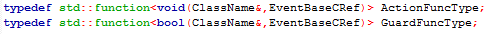
\includegraphics[width=0.8\textwidth]{ft.png}
\caption{Függvény típus definíciók}
\label{fig:ftbgd}
\end{figure}
A típus definíció az állapotgép táblázatban kerül felhasználásra.

\subsection{Állapotgép elkódolás}

Most már minden szükségese elem rendelkezésre áll, hogy az állapotgépet elkódoljuk valamilyen adatszerkezet segítségével. A futási sebességet és az átláthatóságot, valamint az állapotgép felhasználását szemelőt tartva a választott adatszerkezetünk egy hasított asszociatív tömb lesz, ami több azonos kulcsú értéket, azonos esemény eltérő feltétel adott állapotból, esetén is helytálló. A hasításnak köszönhetően az indexelés gyorsan történik és nem okozza a rendszer lassulását. A tömb kulcs értéke egy pár lesz, aminek tagjai az állapot és az abban értelmezett esemény. Az érték szintén egy pár, ami az átmeneti feltételt és a végrehajtandó akciót tartalmazza. A könnyű használhatóság érdekében az érték párban szereplő hivatkozások mindig érvényesek kell legyenek, ezért az állapotgép ősosztályba bevezetünk egy alapértelmezett feltételt, ami mindig igazat ad vissza, lást 3.2 ábra. Az akciók meglétét az állapot váltás megoldása biztosítja, amit később említünk. A C++ban történő implementáció és feltöltés a következőképpen néz ki:

\begin{figure}[hbtp]
\centering
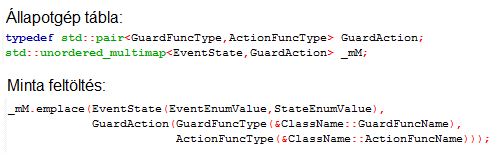
\includegraphics[width=0.9\textwidth]{tbf.png}
\caption{Állapotgép tábla definíció és feltöltés minta}
\label{fig:atgdb}
\end{figure}


Az implementálásnál problémát okoz a kulcs érték pár hasítása, mivel a nyelv nem rendelkezik hozzá beépített hasító algoritmussal, így egy saját megoldást kell definiálnunk. Mivel mind az állapotot, mind az esemény felsorolásként definiáltuk, amit egész számként használunk fel, elég egy két egész számot ütközés nélkül hasító eljárást keresnünk. A megoldást a bitenkénti kizáró vagy művelet biztosítja számunkra. A {\it hash} osztály C++-beli implementáció az alábbi képen látható.

\begin{figure}[hbtp]
\centering
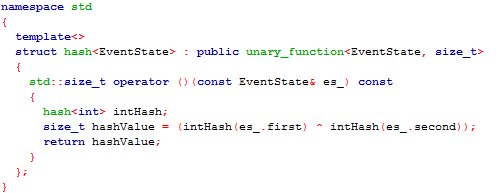
\includegraphics[width=0.9\textwidth]{hashc.png}
\caption{Hash osztály}
\label{fig:hod}
\end{figure}

Az osztályt az STD névtérben definiáljuk így a fordítás során a tömbünk megtalálja további beavatkozás nélkül.

\subsection{Algoritmusok}

Az eddig leírtak segítségével el tudunk kódolni egy állapotgépet a működtetéséhez, azonban szükségünk van még esemény kezelő és állapot váltó algoritmusokra, amik illeszkednek az általunk választott ábrázolásmódhoz. A gép állapotváltásokkal old meg problémákat, tehát először definiáljuk az állapot váltást.

\subsubsection{Állapot váltás}
Mivel az aktuális állapotot egy {\it integer} típusú változó segítségével tartjuk számot az állapot váltó eljárásunk bemeneti paramétere is egy egész szám lesz az állapot felsorolási típusból. Az eljárás törzsében át kell állítanunk az aktuális állapot változót és meghívni az új állapot belépési akcióját. A belépési és kilépési akciókat az állapotgéppel ellentétben nem adatként kódoljuk el, hanem {\it switch} utasítás segítségével az {\it entry} és {\it exit} függvény törzsében.

A logikaként történő ábrázolás mögött két indok áll:
\begin{itemize}
\item {\bf Az ilyen akciók mennyisége}: A modellezési módszertan függvényében az ilyen eljárások száma változó, egyes módszertanok %(???Harrel??? hivatkozás is a könyvre)
csak ilyen akciókat használ és az átmeneteket üresen hagyja, míg mások vegyesen vagy egyáltalán nem alkalmazzák őket.
A dolgozatban a vegyes használat optimalizálása mellett döntöttünk, ekkor a belépési és kilépési akciók száma elenyésző az átmeneti akciókhoz képest.
\item {\bf A fordító program intelligenciája}: Mint azt már leírtuk, a fordító programok sok esetben automatikusan ugró táblára alakítják az értékválasztó utasításokat, ezért ebben az esetben az automatikus optimalizációra bízzuk magunkat.
\end{itemize}
A leírtak alapján az állapot váltó függvény kódja és az {\it entry} függvény a következőképpen néz ki.

\begin{figure}[hbtp]
\centering
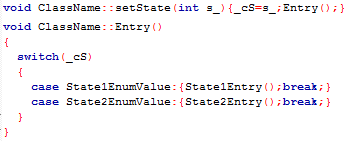
\includegraphics[width=0.6\textwidth]{stent.png}
\caption{SetState és minta Entry}
\label{fig:stmn}
\end{figure}

Ezt a megoldást csak egyszerű állapotok esetén alkalmazhatjuk. Amint rendelkezünk legalább egy összetett állapottal az eljárásnak kezelnie kell az összetett állapotot jelző hivatkozás beállítását is a függvény szignatúra megváltoztatása nélkül.
Az összetett állapotainkat egy asszociatív tömbben tároljuk el, aminek a kulcsa az állapot felsorolási típus egy eleme. A tömbben történő kulcs keresés segítségével így gyorsan meg tudjuk határozni, hogy egyszerű vagy összetett állapotba léptünk be és összetett állapot esetén egy gyors hivatkozás beállítás, valamint állapot inicializálás hozzáadásával a függvényünkhöz már kész is vagyunk. Az kibővített függvényünk egy lehetséges implementációja a 3.7-es ábrán látható.

\pagebreak 

\begin{figure}[hbtp]
\centering
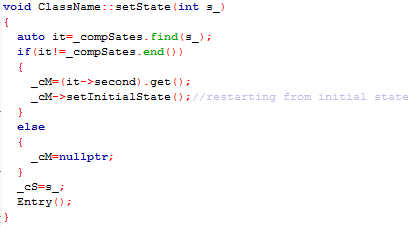
\includegraphics[width=0.68\textwidth]{setsos.png}
\caption{Összetett SetState}
\label{fig:ostmn}
\end{figure}

\subsubsection{Esemény feldolgozás}

Az állapotgépünk felhasználhatóságához szükséges utolsó eljárás a külső felek interakcióját is biztosító esemény feldolgozó függvény. Az események többalakú definíciója biztosítja számunkra az egységes feldolgozó felületet, aminek egy konstans bemenő paramétere az esemény ősosztály. A feldolgozás itt is két részre válik szét:
\begin{itemize}
\item Egyszerű állapotokat tartalmazó gépek.
\item Legalább egy összetett állapotot tartalmazó gépek.
\end{itemize}
Az egyszerű esetben használt algoritmus mind a két esetben a végrehajtás magját képezi. Az algoritmus lépései a következőek:
\begin{enumerate}
\item A bejövő esemény típusa és az aktuális állapot alapján kigyűjtjük a lehetséges átmenetek halmazát az állapotgép táblázatból.
\item Ezután elkezdünk iterálni az átmenetek halmazán.
\item Az első olyan átmenet esetén, ahol az átmenti feltétel teljesül végrehajtjuk a kilépési akciót, majd az átmenti akciót.
\item Amennyiben találtunk olyan átmenetet, amit végre tudtunk hajtani, igaz értékkel térünk vissza különben hamissal.
\end{enumerate}
Az algoritmus szemmel láthatóan nem tartalmaz az állapot váltásra vonatkozó lépést. Ennek oka az állapotgép tábla elkódolásánál nyújtott biztosíték, miszerint mindig létezik átmeneti akció. Ugyanis üres akció esetén is az akció maga az állapot váltás. Az állapot váltás az átmeneti akció utolsó művelete minden esetben. Vagyis, mi az állapot változtatást az átmenti akció részeként értelmezzünk. Az átmenti akciókban az aktuális esemény kinyerését egy gyors konverzióval oldjuk meg, ha szükséges. Az esemény kezelő függvény logikai visszatérési értékére az összetett állapot miatt van szükség. Más esetben a visszatérési érték figyelmen kívül hagyható. Az algoritmus egy lehetséges C++ implementációja az alábbi képen látható egy minta átmenet függvénnyel.

\begin{figure}[hbtp]
\centering
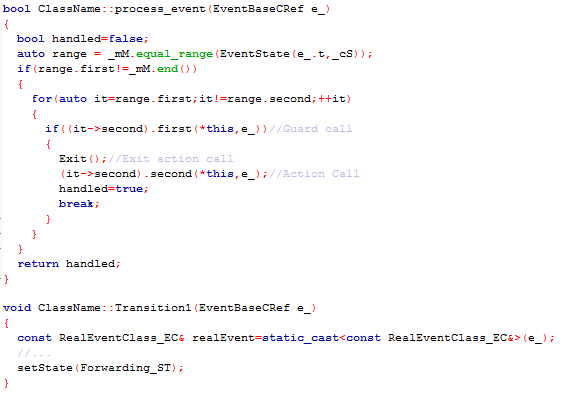
\includegraphics[width=1\textwidth]{specat.png}
\caption{Esemény feldolgozó függvény és minta átmenet}
\label{fig:esp}
\end{figure}

Az összetett esetben a fentebb leírt algoritmust megelőzi egy összetett állapotot kezelő szegmens, ami átveszi a fentebb látható algoritmus helyét az esemény feldolgozó eljárásban. Ennek a megoldásnak a lépései a következők:
\begin{enumerate}
\item Ha összetett állapotban vagyunk, meghívjuk az összetett állapot objektum esemény feldolgozó függvényét az aktuális esemény paraméterrel.
\item Ha egyszerű állapotban vagyunk vagy az összetett állapotban nem tudtuk lekezelni az eseményt, akkor végrehajtjuk az egyszerű esetben leírt algoritmust.
\item Az eljárás végén ha valahol, vagy az összetett állapotban, vagy az aktuális szinten sikerült feldolgoznunk az eseményt, igazzal térünk vissza különben hamis az eredmény.
\end{enumerate}
Az algoritmus egy lehetséges implementációja C++-ban a következőképpen néz ki.

\begin{figure}[hbtp]
\centering
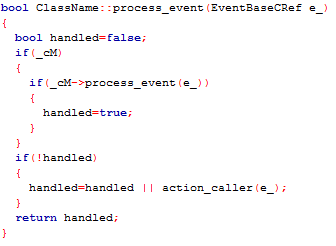
\includegraphics[width=0.6\textwidth]{ospec.png}
\caption{Összetett feldolgozó függvény}
\label{fig:peac}
\end{figure}
A képen látható {\it action\_caller} függvény tartalmazza a másik algoritmust.

Az esemény feldolgozó függvény segítségével az állapotgépekből történő kódváz generálás teljes. A generált kód felhasználható futtatási környezet nélkül is a felhasználó igényei szerint az akció függvények törzsének feltöltésével vagy a kód további kézzel történő módosításával.
Az aktivitások generálásával a következő fejezetben foglalkozunk.

\section{Aktivitás generálás}

Az állapotgépekből történő kódgenerálásról és annak lehetőségeiről több munka is található, mint azt az irodalmi áttekintésben is láthattuk. Az aktivitás diagramokról azonban kevés munka értekezik. Az írások vagy magának a diagramnak a hibát, lehetőségeit vizsgálják, vagy összehasonlítják a módszert a Petri-hálókkal\cite{murata1989petri}. Az aktivitás diagramok használatának hiányát a grafikus ábrázolásmódnak is köszönheti. A kódgenerálást biztosító eszközök inkább definiálnak egy saját akció nyelvet mint, mint hogy ezzel a területtel kelljen foglalkozniuk. Az UML szabvány részeként azonban a kódgenerálás támogatása fontos lehet az általánosság érdekében. Mielőtt a generáló algoritmusok leírásába kezdünk vizsgáljuk meg, mi mit tekintünk egy szabványos UML aktivitás diagram leírásnak.

\subsection{Aktivitiás szerkezeti szabályok}

Az aktivitás diagram egy gráf, ami minden esetben tartalmaz két speciális csúcsot a kezdeti és vég pontot. A gráf minden éle, kivétel a bejövő paraméterekből indulók, a kezdeti csúcsból indul ki és a gráfban minden csúcsából vezet út a vég csúcsba. A köztes csúcsok a speciális csúcsok kivételével, egy kimenő élet tartalmaznak. A bemenő élek száma változó az egyes csúcstípusok esetén. Speciális csúcsnak minősülnek a különböző úgynevezett pszeudo csúcsok, amiknek a segítségével a vezérlési szerkezeteket tudjuk megvalósítani. Az ilyen csúcsok segítségével tudunk továbbá kimenő éleket többfelé szétválasztani, vagy több élet egyesíteni. A pszeudo csúcsoknak többféle felhasználásával is le tudunk írni vezérlési szerkezeteket, ezért mi definiáljuk, hogy az egyes szerkezeteket milyen módon kell megvalósítani, hogy a későbbiekben az algoritmusaink tudjanak támaszkodni ezekre a szerkezeti információkra. Az éleket összegyűjtő {\it join} és szétválasztó {\it fork} csúcsokra nem teszünk megkötést. Az ilyen csúcsok csak a diagram átláthatóságát befolyásolják, generálás során nem igényelnek külön figyelmet. Az elágazásokat és a ciklusokat a {\it decision node} nevű csúcs segítségével írhatjuk le. Az elágazások esetén a {\it decision node}-ból kimenő összes út egy {\it merge node} nevezetű csúcsba kell vezessen.
Amennyiben az ilyen csúcsból nem minden út a megjelölt végcsúcs típusban végződik akkor, vagy hibás az aktivitásunk, vagy ciklust ír le. A ciklus esetén szintén minden él egy a már fentebb említett típusú csúcsból kell induljon ellentétben az elágazással azonban a utak vagy kört írnak le, vagy egy és csak egy esetben az út az aktivitást záró csúcsban végződik. Az élek mindegyikéhez tartoznia kell egy feltételnek, egy élnek pedig vagy üresnek vagy különben feltételnek kell lennie biztosítva ezzel az aktivitás tovább haladását minden esetben. A vezérlési szerkezetek részgráfja tartalmazhat további beágyazott vezérlési szerkezeteket az itt lefektet szabályoknak megfelelően. A ciklusra egy példa a 3.10-es ábrán látható. Az elágazások szerkezetét a 3.11-es árba szemlélteti.

\pagebreak

\begin{figure}[hbtp]
\centering
\includegraphics[width=0.8\textwidth]{activ.png}
\caption{Egyszerű ciklus}
\label{fig:acgt}
\end{figure}

\begin{figure}[hbtp]
\centering
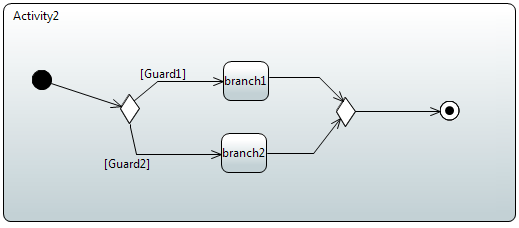
\includegraphics[width=0.8\textwidth]{ifelse.png}
\caption{Egyszerű Elágazás}
\label{fig:aftgt}
\end{figure}

Amennyiben az aktivitás diagram megfelel az imént leírt szabályoknak a kódgeneráló algoritmusok ekvivalens működésű kódot generálnak belőle a cél nyelven. A dolgozatban a cél nyel C++, de az algoritmusok működnek más, nem funkcionális nyelvek esetén is.

\subsection{Algoritmusok}

A diagram szerkezetének leírása után most a felhasználható elemekkel és az azokból történő utasítás készítéssel foglalkozunk. Mivel az egyes elemek különböző utasításokat jelölnek, ezért mindegyikhez külön feldolgozási lépések sorozata szükséges. A feldolgozási lépések azonban jól meghatározhatóak és építőelemként fel tudjuk őket használni az egyes típusok esetén a kódismétlést és karbantarthatóságot ezzel a minimálisra csökkentve. A szükséges algoritmusok a következő feladatokat végzik el:
\begin{itemize}
\item { Paraméter típusának meghatározása}
\item { Paraméter típusának a neve}
\item { Paraméter elérési útvonalának a meghatározása}
\item { Paraméter tulajdonosának a típusának a meghatározása}
\item { OCL kifejezés feldolgozása}
\end{itemize} 
Az utolsó ponttól eltekintve a többi esetben mindig ugyan úgy járunk el apróbb eltérésektől eltekintve. Az utasítások láncként épülnek fel az egyes elemek segítségével. A mi dolgunk ennek a láncnak a visszafejtése addig, amíg el nem érjük a kívánt információ forrását. Ezt egy egyszerű rekurzív lépkedő algoritmus segítségével oldjuk meg, ami ha elért egy forrás csúcs típusú vagy OCL-t tartalmazó elemet megáll és visszatér az eredménnyel. A forrás csúcsok a következőek: 
\begin{itemize}
\item Aktuális objektum hivatkozás ({\it ReadSelfAction}).
\item Aktivitás paraméter csúcs ({\it ActivityParameterNode}).
\item Objektum létrehozási csúcs ({\it CreateObjectAction}).
\item Adattag kiolvasás ({\it ReadStructuralFeatureAction}).
\item Értéklétrehozás ({\it ValueSpecificationAction}).
\item OCL kifejezés csúcs ({\it OpaqueAction}).
\end{itemize}
A visszatérési eredmény, hol a típus, hol a változónév lehet.

Az építő algoritmus leírása után most foglalkozzunk a különböző kifejezéseket leíró csúcsokkal és azok feldolgozásával. Az aktivitások ugyan olyan utasításokat tartalmazhatnak, mint egy írott programozási nyelv:
\begin{itemize}
\item Értékadás ({\it AddStructuralFeatureValueAction}).
\item Érték kiválasztás ({\it ReadValueAction-s}).
\item Változók létrehozása ({\it CreateAction-s}).
\item Konstansok használata ({\it ValueSpecificationAction-s}).
\item Függvény hívások ({\it CallAction-s}).
\item Szignál küldések ({\it SendSignalAction}).
\item Feltételes utasítások és ciklusok használata ({\it DecisionNode-s}).
\end{itemize}
Az utasítások az aktivitás gráfban fák(kivétel a ciklust és az elágazást), amiknek a gyökere az utasítást meghatározó csúcs. A gyökérből induló ágak mennyisége a szükséges információk szerint változó lehet. A 3.12-es ábrán látható pirossal kiemelve egy értékadás utasítás fája, az érték ég OCL-el van megadva, ezért csak egyágú a fánk.

\begin{figure}[hbtp]
\centering
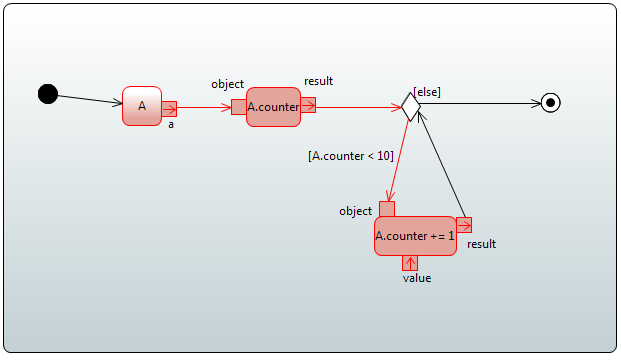
\includegraphics[width=0.8\textwidth]{utpl.png}
\caption{Értékadás fa}
\label{fig:etdsada}
\end{figure}

Az egyes utasításokhoz a következő információkat kell kinyernünk az ágakból:
\begin{itemize}
\item {\bf Értékadás}: bal érték nevének, esetleg típusának meghatározása, ha egy újonnan létrehozott változónak adunk értéket.
\item {\bf Érték kiolvasás}: változó és annak elérési útvonala.
\item {\bf Változó létrehozás}: változó típusa és neve.
\item {\bf Konstans érték létrehozás}: maga a konstans érték.
\item {\bf Függvény hívások}: függvény neve, az elérési útvonala, bemenő paraméterek értéke.
\item {\bf Szignál küldés}: célpont neve, elérése, küldendő szignál típusa.
\end{itemize}

Az elágazások és a ciklusok feldolgozására összetettebb eljárásra van szükség, mivel ezek további utasításokat tartalmazhatnak, továbbá mind a kettő ugyan abból a csúcs típusból indul ki. Mivel mi a fejezet elején az aktivitások szerkezeti leírásánál megkötöttük a két vezérlési szerkezet formai jellemzőit, már csak fel kell használnunk ezt az információt a feldolgozó algoritmusok megírásánál. A feldolgozást végző algoritmus a következő lépéseket végzi el:
\begin{enumerate}
\item {\bf Megnézzük, hogy ciklus-e a szerkezet}: Veszünk minden kiinduló élet és addig lépkedünk rajtuk, amíg vagy el nem érjük a kiinduló csúcsot a ciklus kezdő csúcsot, vagy el nem érjük az aktivitást záró csúcsot. Ha csak egy olyan él van, ami az aktivitást záró csúcsba vezet akkor elégazás a szerkezet, különben ciklus.
\item {\bf Ha ciklus a szerkezet}: Megkeressük az aktivitás végcsúcsába vezető élet, ha tartalmaz feltételt akkor a negálásával megvan a ciklus feltételük, ha nem akkor a többi élről vesszük a feltételeket és az összeéselésükkel kapjuk a ciklus feltételt. Ezután a kivezető élet már nem vesszük figyelembe a feldolgozás során. Ha több él vezet a ciklusba több feltétellel, akkor elindítunk egy elágazás feldolgozást, különben az aktivitás feldolgozó algoritmusunkat használjuk a ciklus csúccsal mint aktivitás kezdő és végponttal.
\item {\bf Ha elágazás a szerkezet}: Megkeressük az elágazást záró csúcsot, aminek a típusa {\it merge node}. Elkezdünk végigmenni a kimenő élek listáján. Az éleken szereplő feltételek az ág feltételek (lehet többszöri elágazás is). Az elágazás törzsének feldolgozására elindítunk egy aktivitást feldolgozó algoritmust az elágazás kezdő és vég csúccsal mint paraméterrel.
\end{enumerate}
A fentebb leírt algoritmus többször hivatkozik az aktivitást feldolgozó algoritmusra, amit eddig még nem írtunk le így most annak a leírása következik. 

Az aktivitás feldogozás valójában egy szélességi gráfbejárás, ami egy megadott kezdeti csúcstól halad egy megadott végcsúcsig.
A bejárás közben megvizsgáljuk, hogy egy csúcs utasítás csúcs-e(a fentebb leírtak egyike), ha igen alkalmazzuk rá az adott utasításhoz szükséges eljárásokat, ha nem figyelmen kívül hagyjuk és folytatjuk a bejárást. Ha feldolgoztunk egy utasítást akkor a részfáját feldolgozottnak jelöljük. A bejárás megáll, ha elérte a megadott záró csúcsot, vagy ha már nincs több olyan csúcs amit még nem dolgozott fel. A bejárás minden a gráfban szereplő utasításból csak egyszer generál kódot.
A mellékelt programban az {\it ActivityExport} fájlban található függvények egy lehetséges megvalósítását tartalmazzák a leírtaknak Eclipse EMF\cite{euml} modelleken.

\section{Futtatási környezet}

Az állapotgépek a kódgenerálás után már futtathatóak, de ahhoz hogy a modellt, amiből a kódot generáltuk teljes egészében fel tudjuk használni szükségünk van egy környezetre, ami sorban kezeli a beérkező eseményeket. A generált kód csak egy olyan feldolgozó függvényt tartalmaz, ami az aktuálisan paraméterben átadott eseményt feldolgozza és visszatér annak függvényében, hogy sikeres volt-e a feldolgozás, volt-e megfelelő átment, vagy eldobtuk az eseményt. A legtöbb állapotgép leíró könyvtár is csak egy ilyen feldolgozó függvényt nyújt számunkra, azonban ez nekünk nem elég. Ahhoz, hogy az állapotgép működése megfeleljen az UML szabványban leírt viselkedésnek szükségünk van egy esemény sor kezelő megoldásra, ami meghívja a generáláskor definiált függvényünket. Ahhoz, hogy egy teljes modellt le tudjunk szimulálni az állapotgépeinknek párhuzamosan egymás mellett kell működnie. 

A célunk tehát egy olyan futtatási környezet tervezése amivel az esemény küldések által vezérelt modell szimuláció lehetségessé válik. A futtatási környezet feladata az eseménysor kezelése és a beérkezett események végrehajtása, valamilyen párhuzamos módon, illetve adunk egy determinisztikus egy végrehajtási szálon történő feldolgozási lehetőséget is. A feladat meghatározása után vegyük sorra mire van szükségünk az általános megoldás megadásához, ami akár más nyelveken is lekódolható és tetszőleges megvalósítású állapotgép illeszthető hozzá a megfelelő leszármaztatások után. A szükséges elemek tehát a következőek:
\begin{itemize}
\item {\bf Futtatási környezet}, ami biztosítja az állapotgépek párhuzamos és egy esetben egyszálú futását.
\item {\bf Állapotgép ősosztály}, amiből a környezetben használni kívánt állapotgépeknek le kell számazni és meg kell valósítani a szükséges kezelő műveleteket.
\item {\bf Esemény ősosztály}, amivel a környezetben egységesen tudjuk kezelni a különféle állapotgép megvalósítások eseményeit. 
\end{itemize} 
Most vizsgáljuk meg részletesen az egyes elemeket és a tőlük elvárt funkcionalitást.

\subsubsection{Futtatási környezet kezelő felülete}
A futtatási környezet feladata az állapotgépek eseménykezelésének a valamilyen módon történő kezelése. Ez a legtöbb esetben valamilyen szálkezelési párhuzamos megoldást takar. A környezetnek biztosítania kell az állapotgépek inicializálását ha szükséges és utána az események feldolgozását a kapott állapotgépeknél. A környezet nem automatikusan indul, el kell indítani és ezután le lehet állítani. A futtatott állapotgépeket a környezet nem birtokolja, ezért azoknak a létrehozását és törlését nem feladata elvégezni. Ezek mellett a szabályok mellett az alábbi funkcionalitást kell a felhasználó felé biztosítanunk:
\begin{itemize}
\item Állapotgépek átadása a környezetnek.
\item Állapotgépek inicializálása, ha szükséges és nem történt meg az átadás előtt.
\item Futtatás indítása.
\item Futtatás leállítása.
\end{itemize} 
Az egyszerű bővíthetőség érdekében a fentebb leírt funkciókat egy interfészben foglaljuk össze és a különböző módon futtató környezeteket külön osztályként valósítjuk meg, így a felületen keresztül történő hivatkozás segítségével bármelyik futtatási módot választhatjuk a megfelelő környezet objektum létrehozásával. Egy programban több különálló környezet is futhat, de azok között semmilyen interakció nem biztosított a környezetek minden esetben függetlenek egymástól. Az interfész egy lehetséges C++ implementációja a 3.13-as ábrán látható.

\pagebreak

\begin{figure}[hbtp]
\centering
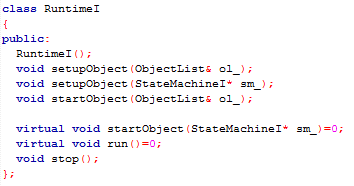
\includegraphics[width=0.6\textwidth]{runtimei.png}
\caption{Futtatási környezet interfész}
\label{fig:runit}
\end{figure}

\subsubsection{Esemény ősosztály}

Az esemény ős csak burkoló osztályként szolgál az illesztendő állapotgép könyvtár eseményeihez és rendelkezik egy létrehozáskor kötelezően megadandó adattaggal a cél állapotgép hivatkozással. A hivatkozás az egyik környezet megvalósításhoz szükséges, valamint a későbbi bővíthetőségi megfontolások miatt amikről később beszélünk. Az esemény ősosztály a 3.14-es ábrán látható.

\begin{figure}[hbtp]
\centering
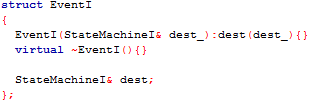
\includegraphics[width=0.58\textwidth]{eventi.png}
\caption{Esemény ősosztály}
\label{fig:esnit}
\end{figure}

\subsubsection{Állapotgép ősosztály}

Az állapotgép ősosztálynak az eseménykezeléshez és az állapotgép inicializáláshoz szükséges műveleteket és adattagokat kell tartalmaznia. Minden állapotgép rendelkezik egy eseménysor hivatkozással és annak kezelésére szolgáló műveletekkel. A tetszőleges állapotgép illesztéshez a felhasználónak két műveletet kell megvalósítania:
\begin{itemize}
\item Az eseményfeldolgozó függvényt.
\item Az állapotgép inicializáló függvényt.
\end{itemize}
Az esemény feldolgozó függvényben le kell kérni a sorból a következő eseményt átalakítani azt a megfelelő típusra és utána tovább adni a külső könyvtár eseményfeldolgozójának, ezután pedig törölni a kivett üzenetet. Az inicializáló függvény az állapotgépet kezdeti állapotba kell hogy állítsa meghívás esetén. 

Most már minden elemről leírtuk a feladatát és szükséges műveleteit, hogy tetszőleges programozási nyelven meg lehessen valósítani valamilyen futtatási környezetet.

\subsubsection{Esemény ősosztály állapotgép paraméter}
Az esemény ősosztályban szereplő cél állapotgép hivatkozás az egyszálú megvalósításhoz szükséges. Ebben az esetben a futtatási környezet tartalmaz egy eseménysort, amire az állapotgépek hivatkoznak. A környezet futtató függvénye egy ciklus, ami megpróbál elemeket kivenni a sorból, ha talál kiveszik és meghívja a cél feldolgozó függvényét az eseménnyel. A megvalósítás egy másik lehetséges módja, ha külön sorban tároljuk a célokat és a küldő függvény kap plusz egy paramétert, ami a célt tartalmazza. A választás azért erre a megoldásra esett, mert az esemény több szinten is jelen van a rendszerben, míg ha külön sor lenne az csak a futtatási környezetben elérhető és további kényelmetlenséget jelentene az elérhetővé tétele különböző szinteken. 

A dolgozathoz három környezetet biztosítunk, egyet, ami minden állapotgépet külön szálon futtat, egy {\it threadpool}-os megoldást, ami egy meghatározott számú szálat oszt ki és váltogatja az aktív állapotgépeket és egy egyszálú megoldást, ami egy eseménysort tartalmaz nem pedig állapotgépenként egyet és sorban hajtja végre a beérkezett eseményeket a céljukon.

\chapter{Eredmények összefoglalása}

A dolgozatban leírt elmélethez tartozik egy megvalósító program, amiből a korábbi fejezetek minta implementációi származnak. A program több modellen is tesztelve lett, hogy a generáláshoz leírt algoritmusok helyes kódot generálnak-e. A generált kód a teszt modellek esetén jelentésben megegyező utasításokat tartalmazott az UML-beli modellel. A generálási folyamat gyors és nem igényel nagy erőforrásokat. A legnagyobb tesztelt működő modell körülbelül 18 állapotgép osztályt több mint 50 aktivitás diagramot, amik átlagosan több mint 10 csúcsot tartalmazott plusz a segéd osztályok. A kódgenerálás körülbelül 2 másodpercet vett igénybe. Amennyiben a forrás UML modell betartotta a leírt szabályokat, a generált kód fordítása sikeres volt. A generált kód tömör lett még a nagyobb aktivitás diagramok esetében is. A több mint 30 csúcsit tartalmazó aktivitásból az algoritmusok egy 10 soros C++ kódot generáltak. A generált kód nem optimalizált, ha az aktivitás diagram tartalmaz felesleges utasításokat azt a C++ kód is tartalmazza. Ezeknek az eltávolítása nem volt kitűzött feladat és a generálás után is végrehajtható egy másik ilyen célú eszközzel. A generált kód továbbá nincs kinézetileg formázva, nem tartalmaz behúzásokat, de a külön utasítások külön sorban szereplenek. A kód formázása a generálás után már bármilyen eszközzel elvégezhető, ami támogat ilyen jellegű funkciót.

A generálás célja a gyorsan futtatható kód volt, de ezen túl igyekeztünk nem átláthatatlan kódot előállítani, hogyha kézi bővítésre vagy átírásra lenne szükség. Az állapotgépek és osztályok generálása semmilyen esetben nem okozott problémát és könnyen kezelhető problémakörnek bizonyult, köszönhetően a bőséges irodalomnak-e téren. Az aktivitásokból történő generálás több tesztelést és kísérletezést igényelt az irodalmi kutatómunka után is, mivel a terület nem rendelkezik igazán jó publikus algoritmusokkal. A futtatási környezet előállítása sem ütközött nehézségekbe a terület dokumentáltságának, és a modern programozási nyelvek által kínált könyvtáraknak köszönhetően.

\subsection{Mérések}

A generált kód hatékonyságának további értékeléséhez összehasonlításként felhasználjuk az irodalmi áttekintésben leírt két állapotgép leíró könyvtárat a Boost::MSM-et és a Boost::Statechart-ot. Az összehasonlítást három szempont alapján végezzük:
\begin{itemize}
\item Futási sebesség.
\item Memória használat.
\item Programkód olvashatóság, átláthatóság.
\end{itemize}
Ugyan az utolsó szempont nem mérvadó, mivel a kód generált a mi esetünkben, de bizonyos esetekben szükséges lehet a felhasználói módosításra, javításra vagy akár csak a generált kód megértésére. A futási idő és a memória felhasználás vizsgálatára a gépterem %hivatkozás
példa egyszerűsített változatát használjuk fel és implementáljuk (illetve generáljuk) az egyes könyvtárakkal.

Az egyszerűsített példa a következő: Van egy géptermünk, ami csak adott mennyiségű számítógéppel rendelkezik. A termet a tanulók használják bizonyos időközönként. A teremnek három állapota van:
\begin{itemize}
\item Üres.
\item Vannak bent.
\item Tele.
\end{itemize} 
Ha a terem üres vagy nincsen tele akkor a hallgatók bemehetnek, különben sorban kell állniuk. 

\pagebreak

A tanulóknak szintén három állapota van:
\begin{itemize}
\item Dolgozik.
\item Sorban áll.
\item Géptermet használ.
\end{itemize}
Mivel az üzenetküldéseket és az állapotváltásokat szeretnénk vizsgálni ezért nem használunk időzítőket, hanem minden tanuló rendelkezik egy számlálóval ahányszor a gépterembe próbál menni és utána leáll. A szimuláció akkor ér véget ha minden hallgató elérte a kívánt gépterem használatot. A tanulók száma mindig több mint a gépterem maximális kapacitása. A mérésekben a gépterem maximális kapacitását 100 főre rögzítjük, a használati számot pedig 1-re rögzítjük és a termet használni kívánó hallgatók számát paraméterezzük. 

A mérésekhez felhasznált számítógép a következő paraméterekkel rendelkezik:
\begin{itemize}
\item Memória: 4 GB PC3-10600 DDR3 SDRAM @ 1333MHz
\item CPU: Intel(R) Core(TM) i5-2450M CPU@ 2.50Ghz 2.50Ghz
\item Operációs rendszer: MS Windows 7 64-bit
\end{itemize}

Több mérést is futtatunk, ahol a tanulók száma tízezres nagyságrendeknek felelt meg és a következő futtatási eredményekre jutottunk: 

\begin{figure}[hbtp]
\centering
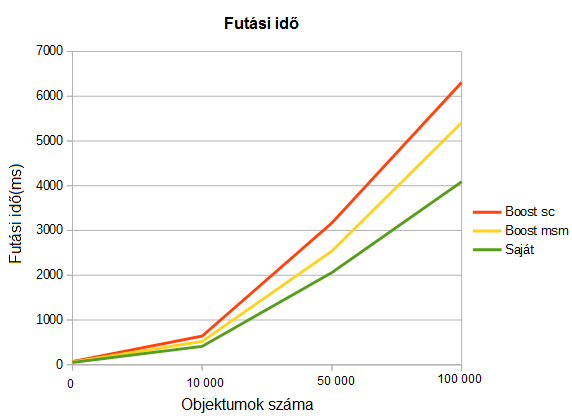
\includegraphics[width=0.7\textwidth]{futasido.png}
\caption{Futási idő mérések}
\label{fig:ftgs}
\end{figure}

\begin{figure}[hbtp]
\centering
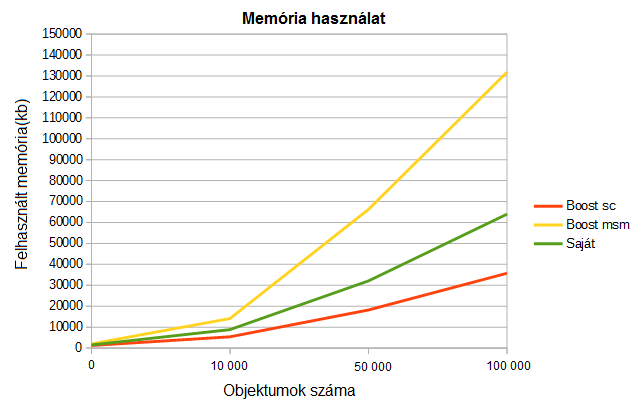
\includegraphics[width=0.7\textwidth]{memoria.png}
\caption{Memóriahasználat mérések}
\label{fig:ws}
\end{figure}

Memória felhasználás terén az általunk választott ábrázolás rosszabbul teljesít mint a Boost::Statechart könyvtár, ami várható volt, mivel az a könyvtár a minimális memória használatot tartja elsődleges szempontnak. A Boost::MSM, ami a futási időre helyezi a hangsúly azonban több memóriát használ fel az objektumok tárolására, mint a dolgozatban leírt ábrázolás. A memória felhasználás terén tehát sikerült javítanunk a hasonló tulajdonságú könyvtáron, azonban azzal a könyvtárral aki ezt tekinti elsődleges szempontnak még így sem tudunk versenyezni.

A futási idő tekintetében a Boost::MSM jobban teljesít mint a Statechar, ami az elvárt viselkedés. Az általunk leírt megoldás azonban, mind a két könyvtárnál jobban teljesít futásidő tekintetében és az objektumok számának növekedésével ez a gyorsulásbeli különbség egyre látványosabban megmutatkozik.
A lemért eredmények alapján tehát sikerült egy gyors, memóriát mértékletesen használó megoldást előállítanunk.

\chapter{Program dokumentáció}

A dolgozatban több helyen is hivatkozunk a leírtakat megvalósító programra, a továbbiakban ennek a programnak a rövid felhasználói és fejlesztői dokumentációját írjuk le.

\section{Felhasználói dokumentáció}

\subsubsection{Szükséges eszközök}

A progarm működéséhez az alábbi eszközökre van szükség:
\begin{itemize}
\item G++
\item Ar
\item make
\item Java 
\end{itemize}
További kényelmi eszközként felhasználható az Eclipse IDE, de nem szükséges.

\subsubsection{Futtatás és Eredmény}

A program parancssorból futtatható a neve és a bemeneti paraméterek megadása után. Két kötelezően megadandó bemeneti paraméter van. Az első egy .uml fájl, ami a modellt tartalmazza a második az exportálás helye. További paraméterként megadhatunk kapcsolókat is:
\begin{itemize}
\item {\bf -h} vagy {\bf -help}: Ha nem adunk meg semmilyen paramétert csak ezt a kapcsolót a program kiír egy rövid használati utasítást
\item {\bf -rt}: A generált kód a futtatási környezetet is tartalmazza (a runtime mappában) a szükséges leszármaztatásokkal. A main.cpp fájl leír egy minta használatot. A környezet használatához külön le kell azt fordítanunk és statikusan linkelnünk a többi fájl fordításához. A generált make fájl használata esetén a statikus könyvtár {\it libsmrt} néven elkészül és linkelődik a fordítás során. 
\item {\bf -cdl}: A generált kód minden átmeneti akciója kiírja a nevét, amikor meghívódik, ha a fordítássorán definiálva volt a \_DEBUG makró. A generált make fájl használata esetén a makró definiálásra kerül.
\end{itemize}

A generálás után a fordítást a generált make fájl segítségével végezhetjük el legkönnyebben, ami lefordítja a fájlokat így tesztelvén a generált kód érvényességét is.
A generálás minden esetben létrehoz három darab C++ fájl:
\begin{itemize}
\item {\bf event.hpp}: Az eseményeket és aze esemény ősosztály tartalmazó fájl.
\item {\bf statemachinebase.hpp}: Az állapotgépek ősosztályát tartalmazó fájl.
\item {\bf main.cpp } : Minta használati kódot tartalmaz a {\bf -rt} kapcsoló esetén, különben egy egyszerű kiíratás.
\end{itemize}
Az osztályokból .hpp kiterjesztésű fejállományok és .cpp kiterjesztésű fájlok keletkeznek. Az összetett állapotokból külön osztály keletkezik, aminek a fájl nevei az \_subSM el végződnek. A program intelligens módon generálja le az állapotgép osztályt és csak a szükséges minimális algoritmusokat írja bele a kódba. Vagyis az összetett állapotokat tartalmazó állapotgép műveletek és plusz adattagok csak összetett állapotot tartalmazó gépek esetén kerülnek a generált kódba.

\section{Fejlesztői dokumentáció}

A program java nyelven készült, hogy egységesen lehessen kezelni a projekt többi eszközével. Mivel önálló alkalmazásnak készült, ezért igyekeztünk elkerülni a függőségeket és csak a minimális szükséges Java könyvtárakat használtuk fel. A program egyetlen igazi külső függősége az Eclipse UML2-t leíró plugin-je a {\it org.eclipse.uml2.uml.resources.jar}.

\subsection{A program szerkezeti felépítése}

A program három jól elkülöníthető részből áll:
\begin{enumerate}
\item {\bf Az uml modell bejárás és feldolgozó algoritmusok}: Ez a rész az {\bf export.cpp} csomagban található és három jól elkülönülő részből áll. Az első rész két fájlból áll a {\bf TxtUMLCpp.java} és a {\bf UML2ToCpp.java}-ból, amik a program belépési pontjait és azzal kapcsolatos kiíratásokat tartalmazza és meghívják a bejárást és generálást tartalmazó eljárásokat. A második jól elkülönülő rész az állapotgépek és osztályok generálásával foglalkozik és a {\bf ClassExport.java} fájlban található. A harmadik rész az aktivitásokból történő kódgenerálásért felelős és az {\bf ActivityExport.java} fájlban található. A csomag további tartalma a közös műveleteket írja le. 
\item {\bf A C++ kódgenerálási sablonok}: Ebben a csomagban találhatóak a C++ sablonok, amikbe a megfelelő nevek és típusok behelyettesítése után érvényes C++ utasításokat kapunk. A programnak ez a része bármikor lecserélhető más sablonokra.
\item {\bf Az előre megírt C++ fájlok}: Ebben a csomagban tároljuk a már kész, változást nem igénylő kódokat, mint például az állapotgép ősosztály vagy a futtatási környezet kódja, ami csak átmásolódnak a cél mappába a generálás során.
\end{enumerate}
A három modul jól elkülönül és könnyedén cserélhető. A felhasznált algoritmusok leírása a dolgozat elméleti részében található.

\subsection{Tesztelés}

A programot több modellen is teszteltük fekete doboz módon. A tesztek a következő teszteseteket tartalmazták és eredményt adták:
\begin{itemize}
\item Bemeneti paraméterek számának a hibájának tesztje:
\begin{enumerate}
\item Paraméter nélküli futtatás.
\item Kevesebb paraméter megadása mint elvárt.
\item Több hibás paraméter megadása.
\end{enumerate}
Eredmény: A program hibát jelez és javasolja a segítség nyújtó kapcsolatokkal történő futtatást.

\item Helyes számú, de hibás paraméter megadása:
\begin{enumerate}
\item Hibás fájl elérés: A program az elérési útvonal hibáját jelzi és leáll.
\item Hibás cél könyvtár: A program a cél érvénytelenségét jelzi (nincs jogosultság, nem létező útvonal, ...).
\end{enumerate}

\item Nemlétező kapcsolok megadása a helyes paraméterezés után: A program figyelmen kívül hagyja a hibás kapcsolókat és további paramétereket.
\item Helyes bemenetek megadása különböző helyes modellekkel (elágazást, ciklust, egyszerű állapotgépeket, összetett állapotgépeket tartalmazó) és kapcsolókkal: A generálás és fordítás sikeres.
\end{itemize}

A fehér doboz tesztelés csak helyes modelleken történt, mivel az algoritmusok és a program előfeltétele, hogy a kapott modell megfelel a leírt szintaktikai szabályoknak, amennyiben nem a futási eredmény nem definiált.
A következő fehér doboz teszteket végeztük, a modell tartalmát illetően:
\begin{itemize}
\item Állapotgép nélküli.
\item Egyszerű állapotgépeket tartalmazó.
\item Összetett állapotokat tartalmazó.
\item Egyszerű és összetett állapotokat tartalmazó.
\item Aktivitásban ciklust tartalmazó.
\item Aktivitásban elágazást tartalmazó.
\item Aktivitásban egymásba ágyazott szerkezeteket tartalmazó.
\item A fentebbi pontok kombinációi.
\end{itemize} 
A kódgenerálás és fordítás minden esetben sikeres.

\nocite{*}
\bibliographystyle{ieeetr}
\bibliography{diplomamunka}


\end{document} 


